\section{Methodology}

\subsection{Experimental Pipeline}
The pipeline consists of five stages: data loading and scaling, sequence generation, model training, out-of-sample forecasting, and interpretability analysis. We evaluate multiple design factors using controlled ablation to isolate contribution from architecture, macro features, and optimization.
Figure~\ref{fig:pipeline_overview} summarizes the end-to-end workflow used in this study.

\begin{figure}[H]
\centering
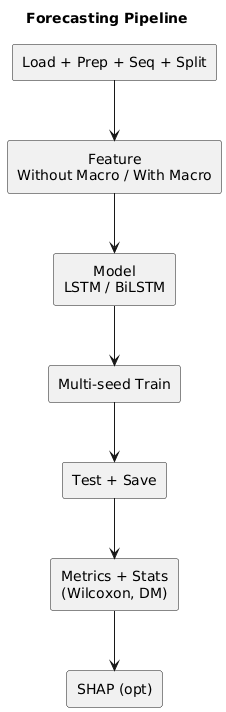
\includegraphics[width=0.90\columnwidth,height=0.45\textheight,keepaspectratio]{images/flowchart.png}
\caption{Compact vertical pipeline overview used for the ablation and evaluation workflow.}
\label{fig:pipeline_overview}
\end{figure}

\subsection{Primary Recurrent Forecasting Framework}
\subsubsection{LSTM and BiLSTM Baselines}
The original recurrent baselines use a single-layer recurrent encoder followed by a fully connected prediction head mapping the final hidden state to a scalar forecast. The shared architectural design ensures that performance differences are attributable to the directionality of temporal encoding rather than depth or capacity changes. The two variants are:
\begin{itemize}
    \item \textbf{LSTM}: unidirectional temporal encoder with hidden size $h$, producing a single forward hidden state of dimension $h$.
    \item \textbf{BiLSTM}: bidirectional temporal encoder with hidden size $h$, concatenating forward and backward states to produce an output of dimension $2h$.
\end{itemize}
Both variants apply a dropout rate of 0.2 between the recurrent layer and the prediction head to mitigate overfitting. The prediction head consists of a single linear layer with ReLU activation, outputting the next-day closing price.

\subsection{Supplementary Architecture Extensions}
\subsubsection{Transformer Extension Models}
We extend the primary recurrent benchmark with Transformer-based sequence models adapted to one-step-ahead stock-price forecasting:
\begin{itemize}
    \item \textbf{Informer}: an Informer-oriented encoder with positional encoding, ProbSparse-style attention, and sequence distilling to reduce long-sequence computation \cite{zhou2020informer}.
    \item \textbf{Autoformer}: an Autoformer-oriented encoder using moving-average decomposition and an Auto-Correlation-style temporal block to separate trend and seasonal components \cite{wu2021autoformer}.
\end{itemize}
For reproducibility, the implementation also keeps lighter Informer-style and Autoformer-style baselines in the codebase. These Lite variants are not the primary Transformer results because they omit the original ProbSparse attention and Auto-Correlation mechanisms.

\subsubsection{Recurrent Architecture Variants}
To test whether the recurrent family can be strengthened without switching to Transformer models, we add ten recurrent variants: LSTM/BiLSTM with pre-normalization, post-normalization, and combined pre+post normalization; CNN-LSTM and CNN-BiLSTM encoders; and LSTM/BiLSTM with temporal attention. The normalization variants apply LayerNorm before and/or after recurrent encoding. The CNN variants apply a one-dimensional convolutional feature extractor before recurrent modeling. The attention variants learn temporal weights over hidden states before the prediction head.

\subsection{Budgeted Hyperparameter Optimization via Genetic Algorithm}
To isolate the effect of hyperparameter tuning from architectural choices, we introduce a constrained search procedure based on a Genetic Algorithm (GA). The GA operates on a fixed computational budget and optimizes three hyperparameters using validation loss as the fitness objective:
\begin{itemize}
    \item \textbf{Hidden dimension} ($h$): searched over $\{32, 64, 128, 256\}$,
    \item \textbf{Learning rate} ($\alpha$): searched over $\{1 \times 10^{-4}, 5 \times 10^{-4}, 1 \times 10^{-3}, 5 \times 10^{-3}\}$,
    \item \textbf{Sequence length} ($L$): searched over $\{10, 20, 30, 60\}$.
\end{itemize}
Each GA individual encodes one $(h, \alpha, L)$ triplet. The population size is set to 8 and the number of generations is fixed at 5, yielding a total evaluation budget of $8 \times 5 = 40$ configurations per case. Tournament selection (size 3) is used for parent selection, and single-point crossover with a per-gene mutation probability of 0.2 is applied. The hand-picked default configuration used in non-GA cases is $(h=64, \alpha=10^{-3}, L=20)$. Configurations tagged as ``\_ga'' in the results tables indicate the GA-optimized setting. This design tests whether budgeted tuning improves accuracy and stability versus fixed defaults, acting as an ablation factor for optimization effort rather than a contribution claim about the search algorithm itself.

For the supplementary Transformer experiments, the code also supports a budgeted random-search mode. This mode uses the same validation objective and a small candidate budget to obtain fast initial estimates before running more expensive GA-style tuning or SHAP analysis.

\subsection{Statistical Validation}
Beyond average error reporting, we apply two complementary tests:
\begin{itemize}
    \item \textbf{Wilcoxon signed-rank test}: a nonparametric paired test applied on seed-level RMSE vectors ($n=5$) to assess whether median performance differences are significant without assuming normality.
    \item \textbf{Diebold-Mariano (DM) test}: applied on aligned forecast-error residuals to evaluate whether one model produces significantly lower prediction errors than another.
\end{itemize}
The Wilcoxon test provides seed-level robustness evidence, while the DM test assesses time-series-level significance. Agreement between both tests strengthens confidence in reported gains.
